\documentclass[10pt, portrait, letterpaper]{article} 

\usepackage{geometry}
\usepackage{graphicx}

\geometry{margin=0.5in}
\graphicspath{{../}}

\title{ECE 3710 Group 3 Control and Decode Report}
\author{Aidan Leary, Trae Hillstead, Woojin Lee, Hayoung Im}

\begin{document}
  \maketitle

  \section{Introduction} 
  This document provides an in-depth overview of the design choices, implementation details, and considerations for developing a functional CR16-based processor. The primary objective of this project up to this point was to design, implement, and test a working processor capable of executing a defined set of baseline instructions, including arithmetic, logical, load/store, and branch operations, as well as jump and link instructions. By integrating the ALU, register file, datapath, memory interface, instruction decoding, and control FSM, the CPU is now able to process and execute instructions on the FPGA.

  \section{FPGA Resource Utilization}
  \begin{itemize} 
    \item Logic Utilization: 591/32070 ALMs (2\%)
    \item Total Registers: 411 
    \item Total Block Memory Bits: 1,048,832/4,065,280 (26\%)  
      \subitem this is with a memory size of $2^{16}$, we will increase this for hosting sound samples
    \item Total DSP Blocks: 1/87 (1\%)
  \end{itemize}

  \section{Custom Intructions} 
  The following is a list of custom instructions.
  \begin{itemize} 
    \item MSCR: reset millisecond counter 
      \subitem takes no args
    \item MSCP: pause millisecond counter 
      \subitem takes immediate value of 0 for no pause or 1 for pause
    \item MSCG: get millisecond count
      \subitem stores count in Rdest
  \end{itemize}

  \section{Design Choices} 
  The following provides an overview of all major modules within the CPU design, and the design considerations that went into making them.

  \subsection{Memory} 
  Nothing major to note about memory, just that we changed to a read on negative edge in order to maintain the two-state FSM design.

  \subsubsection{Memory Mapped I/O}
  Memory mapped I/O is implemented by simply checking the memory address and changing the source of the memory read data or by writing the write data to a register. 
  If the CPU provides an address that points to I/O space, the write data will be written to the appropriate register if write is enabled, 
  and the source of the read data to the CPU will be either be a register, or directly from an I/O device. 
  If the CPU attempts a write to a input I/O device, nothing will happen.

  \subsection{CPU} 
  The CPU module simply instantiates the data path and CPU controller modules. It exposes memory signals, reset, and clock as ports.

  \subsection{Data Path} 
  The data path contains modules that operate on data, or control the path that data takes. 
  All data operations are within submodules, making this module purely a connecting module. 
  This was a deliberate choice, in order to maintain good separation of concerns.
  Each following section describes the important details of each submodule instantiated within the data path module.

  \subsubsection{Muxs}
  For consistency's sake, all muxs are implemented using general purpose modules. There are three muxs, one for the source of the write to the register file, one for the ALU's b port, and one for the memory address output.

  \subsubsection{Register file write mux}
  This mux is 6 inputs wide. The inputs are as follows:
  \begin{enumerate} 
    \item result from ALU 
    \item data read from memory
    \item data read from Rsrc 
    \item extended immediate value
    \item current PC plus one 
    \item millisecond count
  \end{enumerate}

  \subsubsection{ALU Source b mux}
  This mux is 2 inputs wide. The inputs are as follows: 
  \begin{enumerate}
    \item data read from Rsrc 
    \item extended immediate value
  \end{enumerate}

  \subsubsection{Memory address mux} 
  This mux is 2 inputs wide. The inputs are as follows.
  \begin{enumerate} 
    \item data read from Rsrc
    \item extended immediate value
  \end{enumerate}

  \subsubsection{ALU}
  The ALU implements ADD, SUB, AND, OR, XOR, NOT, LSH, ASH, and MUL operations. Since shift amounts are encoded as a two's complement value (positive for left, negative for right), the ALU takes the two's complement inverse of the b input and uses this as the shift amount when the b input is negative. The ALU flags relating to overflow are calculated on ADDs and SUBs, and the flags relating to comparisons are only calculated on SUBs. The zero flag is always calculating, leaving it up to the controller to decide what instructions set this flag.

  \subsubsection{Register File}
  The RF is written to on the rising edge of the clock, and reads combinationally.
  In order to rule out any potential instability related to the combinational 
  read, it may be necessary to move to a sequential read, specifically because 
  there is a data path signal that loops back to the RF for the MOV instructions.

  \subsubsection{PC ALU}
  The PC ALU allows selection of a three different addressing modes for calculating the next PC. 
  These modes are next instruction, offset, and absolute. 
  Next instruction simply increments the PC, offset adds an immediate offset, and absolute 
  jumps to an exact address.
  This module also has an output signal that is always the current PC plus one. 
  This signal is used for writing the PC to the register file during JAL instructions. 
  The additional wire allows for the next PC to be calculated, and stored in the PC register 
  at the same clock edge as the incremented current PC is stored to the register file.

  \subsubsection{Immediate Extender} 
  This module is used to select from a one of three different ways to extend 
  the 8-bit immediate encoded in the lower bits of the instruction to 16-bits.
  These modes are sign extend, zero extend, and align high. 
  The first two modes are self explanatory, and align high shifts the immediate 
  value 8-bits left, zero filling the lower bits. 
  This mode is used exclusively for the LUI instruction.

  \subsubsection{Comparator} 
  This module takes the comparison mnemonic, which is encoded in the Rdest segment of the 
  instruction, and uses it to select an expression to use to evaluate conditionals. 
  This allows the result of a comparison instruction to be represented by a single signal, 
  removing the need to examine the Rdest operand directly in the controller. 
  The controller simply has to use the comparison result signal to decide upon 
  the PC addressing mode necessary to calculate the next PC.

  \subsubsection{PSR} 
  The processor status register is only being used to store the results from the 
  ALU flags. 
  The register is implemented as a full 16-bit width register as defined 
  in the CR-16 architecture, this choice was deliberate to allow for easy 
  expandability to include the other non-ALU flags which are not baseline. 
  Additionally, this model would allow for an easy way to add a signal that allows 
  the PSR to be stored into the register file should it be necessary for an instruction.

  \subsubsection{PC and Instruction Registers}
  The PC and Instruction registers are implemented using a general purpose 
  16-bit register module, inspired by the Mini-MIPS design. 
  The reason for this is because these registers don't have any special 
  attributes like the PSR does where individual bits need to be written 
  independently, making a purpose-built module pointless.

  \subsubsection{Millisecond Counter}
  The millisecond counter is fairly self-explanatory, but the control signals are 
  worth explaining.
  There is a user reset, a pause signal, and a 
  config enable. 
  The config enable allows the pause state to be changed, by latching the pause 
  signal (which is connected to the LSB of the extended immediate) into a 
  register. 
  The user reset resets the millisecond count, but leaves the counter that enables 
  the millisecond count alone. 
  This allows for the millisecond count to remain synchronized even through a reset. 
  An application where this matters is counting seconds, where the CPU will check if 
  the count has reached 1000 milliseconds and then reset it. 


  \subsection{Control FSM}
  The control FSM uses a 2-state design, with fetch and execute as the states. 
  The data path design allows for a lot of work to be done in parallel, enabling this design, as well as the memory being read on the falling edge of the clock. 
  The memory read had to be clocked on the falling edge of the clock due to the need to read data from memory, and write it to registers within one clock cycle.
  Fig. \ref{fig:fsm} shows the two states and their transitions.

  \begin{figure}[h]
    \centering
    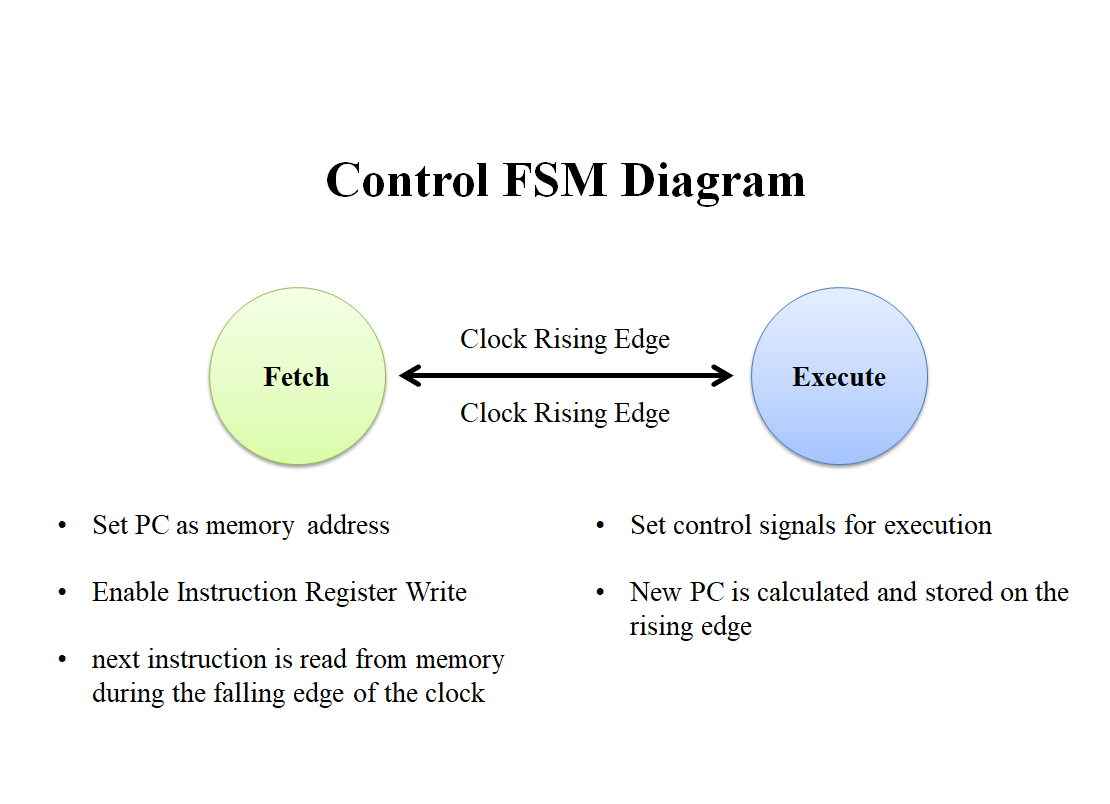
\includegraphics[width=5in]{fsm diagram.PNG}
    \caption{State transition diagram for the CPU controller FSM.}\label{fig:fsm}
  \end{figure}

  \subsubsection{Fetch State}
  During this state, the PC is selected as the memory address, and the 
  instruction register write enable is set high. 
  The next instruction is read from memory during the falling edge of the 
  clock, ensuring that each instruction is latched at the rising edge of the 
  clock as the controller enters the execution state. 
  This ensures that the instruction is readily
  available at the start of each execution state. 

  \subsubsection{Execute State}
  During this state, the control signals for the data path are set, 
  and the result from the instruction will be stored in the 
  register file (if applicable)
  on the rising edge of the clock as the controller leaves this state.
  Instructions such as JAL and BCOND are able to be completed in 
  one state due to the added parallelism of the data path.
  The comparison instructions use the comparison result signal 
  from the data path to decide on a PC addressing mode which is used 
  to calculate the new PC, latched as the FSM leaves this state 
  and the next instruction fetch begins.
  The JAL instruction is able to be completed during this cycle 
  because the PC plus one signal can be stored in the register 
  file while the next PC signal is latched into the PC register.
  Additional design choices that facilitate the parallelism of this state are 
  the memory read on the falling edge of the clock, and the combinational 
  read of the register file.

  \section{Next Steps} 
  There are a few exponents external to the CPU and memory system that we will need. 
  The first is a VGA bitgen component, this will likely be a spin on glyph based graphics. 
  The bitgen component will read from a portion of the memory accessible to the CPU, so that the 
  CPU is able to update the graphics without any special instructions. 
  Additionally, the horizontal and vertical count will be memory mapped so that the CPU can decide when to 
  initiate a refresh of the display.

  The next major component (really several components) is the audio system. 
  The on-board audio codec is already working, as is streaming audio from the HPS ARM core via a Linux application. 
  The rest of the development of this design will focus on mixing audio samples, including playing several 
  audio samples at once, and adding a memory-mapped interface so that our CPU can play/pause the audio.
  
  The VGA bitgen component and audio components will conflict with each other on memory reads, so it will also be necessary 
  to add an extra module connected to the second port of the memory to address this.

  The final component needed is some additional processing on the input from the drum samples. 
  The signal is fairly stable, but a little bit of debouncing will most likely be best.


  \section{Conclusion}
  In conclusion, key design choices, like the modular structure of the datapath and the two-stage control FSM, 
  allow for efficient execution by leveraging parallelism and reducing complexity in our design. 
  Looking forward, the planned augmentations to integrate I/O capabilities, 
  such as memory-mapped addresses for a piezo drum board and VGA display, 
  will allow the CPU to interact with our planned game peripherals. 
  These augmentations are designed to build upon the current framework 
  without significant changes to the datapath or control logic, ensuring an efficient path for further development.

  \subsection{Contributions}: 
  \begin{itemize} 
    \item Aidan 
      \subitem control FSM 
      \subitem memory 
      \subitem ALU, RF, CPU, datapath testbenches
      \subitem ALU 
      \subitem ALU/RF demonstration module
      \subitem millisecond counter 
      \subitem CPU system basic module
      \subitem this report
    \item Trae
      \subitem data path 
      \subitem register file 
      \subitem control FSM
      \subitem ALU/RF demonstration module
      \subitem this report
    \item Woojin 
      \subitem CPU controller testbench 
      \subitem control points list 
      \subitem FSM state diagram in this report
    \item Hayoung
      \subitem ALU 
      \subitem Fibonacci assembly code
  \end{itemize}
\end{document}
